\documentclass{article}

% --- load packages ---

\usepackage[margin=1in]{geometry} % change the margins
\usepackage{amsmath} % useful math environments and commands like align
\usepackage[colorlinks,bookmarks,bookmarksnumbered,allcolors=blue]{hyperref} % hyperlinks between references
\usepackage{graphicx}  % include images
\usepackage[caption=false]{subfig} % subfigures.  false option prevents conflicts in caption styling with other packages
\usepackage{booktabs} % better tables
\usepackage[capitalise]{cleveref} % better referencing. uses cref.
\usepackage[section]{placeins} % sometimes useful to prevent figures from floating out of a section
\usepackage{cite} % handles multiple citations in one command better
\usepackage{doi} % allow correct hypderlinking of DOIs
\usepackage{amssymb}


\graphicspath{{figures/}}
\DeclareMathOperator{\taninv}{\tan^{-1}}
\DeclareMathOperator*{\argmin}{arg\,min}


\begin{document}

\title{Constrained Optimization}
\author{Seth Nielsen}
% put in \date{} if you don't want a date to appear, or enter a specific date, otherwise default is today's date.
\date{}
\maketitle

\section{Introduction}

\section{Project Subproblem}

An important aspect of many autonomous vehicle applications is, given a set of waypoints,
to be able to generate a trajectory that will guide the vehicle through all of the waypoints 
but that is also dynamically feasible. Many algorithms exist to generate trajectories
(RRT, A$^*$, ect.) but these methods do not guarantee that the generated path can be attained
by the vehicle due to constraints on the motion. Techniques, such as differential flatness,
exist to generate optimal paths that satisfy the dynamic constraints giver that certain criteria
are met by the dynamic system. The subproblem that we approach is to use the differential flatness 
technique on a bicycle model to generate a minimum jerk trajectory between two waypoints.

\subsection{Differential Flatness}
A nonlinear system is defined by \cref{eq:xdot} and \cref{eq:y}
\begin{equation}
  \dot{x} = f(x,u),
  \label{eq:xdot}
\end{equation}
\begin{equation}
  y = h(x,u),
  \label{eq:y}
\end{equation}
where $x \epsilon \mathbb{R}^n$ is the system state, $u \epsilon \mathbb{R}^m$ the inputs, $\dot{x}$ the time derivative of the state,
and $y \epsilon \mathbb{R}^p$ the system outputs. The system is differentially flat if there 
are $m$ output functions (called flat outputs) such that all of the states and inputs can be 
expressed in terms of the flat outputs and their derivatives.

At first glance this may not seem helpful but many systems have many more states than they do 
inputs (i.e., $n > m$). What the above definition is saying is that in a differentially flat
system we can take the $m$ desired flat outputs and define the states and inputs as a function 
of these outputs. Defining a trajectory in this way reduces the search space required to 
define the trajectory. We show how this works using the bicycle model in the following subsection.

\subsection{Bicycle/Car Model}

The bicycle is a model that operates in the plane with an $x$ and $y$ position as well as a 
heading angle $\theta$. The inputs to the system are the velocity $v$, and steering angle $\gamma$.
A visual representation of this model can be seen in \cref{fig:bicycle_model}.
The dynamics of the bicycle model are expressed in \cref{eq:car_model} where $v$ and $\gamma$
are the inputs to the system and $l$ is the length between the wheels.

\begin{equation}
  \centering
\begin{aligned}
  \dot{x} = v\,\cos(\theta) \\
  \dot{y} = v\,\sin(\theta) \\
  \dot{\theta} = \frac{v}{l}\tan(\gamma)
\end{aligned}
\label{eq:car_model}
\end{equation}

\begin{figure}[bth]
  \centering
  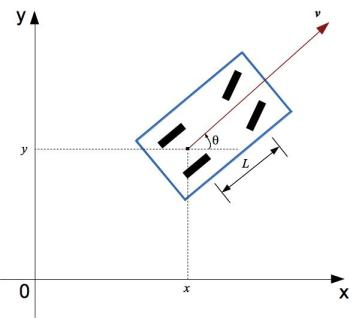
\includegraphics[scale=0.5]{car_model.jpg}
  \caption{Visual representation of the car/bicycle model\label{fig:bicycle_model}}
\end{figure}

The bicycle model is differentially flat where the flat outputs are the desired position denoted as 
$x_d$ and $y_d$. We note that two of our states are the same as our flat outputs meaning that we only
need to derive the third state. \Cref{eq:desired_states} shows each state as a function of the flat outputs.

\begin{equation}
  \begin{aligned}
    x_d = x_d \\
    y_d = y_d \\
    \theta_d = \taninv{\frac{\dot{y_d}}{\dot{x_d}}}
  \end{aligned}
  \label{eq:desired_states}
\end{equation}

Examing \cref{fig:bicycle_model} shows that the derivation of $\theta_d$ is correct in that
it can be derived from the components of the velocity. From the dynamics equations we can solve for the inputs and they can 
be found in \cref{eq:desired_inputs}.

\begin{equation}
  \begin{aligned}
    v = \frac{x_d}{\cos(\theta_d)} \\
    \gamma_d = \taninv{\frac{\dot{\theta}_d l}{v}}
  \end{aligned}
  \label{eq:desired_inputs}
\end{equation}

Note that although $\gamma_d$ does not appear to be a function of the flat outputs, it is a function
of $\dot{\theta_d}$ which is a function of the flat outputs. Since all of the inputs and states are expressed as a function of $x_d$, $y_d$, and 
their derivatives, we have shown that the bicycle model is differentially flat. All that is 
left is to mathematically define a path for $x_d$ and $y_d$ that will take us from out desired 
starting point to end point. This is often done with quitic polynomials, splines or other basis functions.

\subsection{Minimum Jerk Cost Function}

We seek to define a path to minimize the jerk on the vehicle. Minimizing jerk has 
certain benefits such as decreased mechanical wear that is desired. To achieve this
we will use a quintic polynomial to define both $x_d$ and $y_d$ as can be seen in \cref{eq:quintic_polynomial}.

\begin{equation}
  T(t) =\begin{pmatrix}
x_d\\y_d 

\end{pmatrix} = \begin{pmatrix}
p_{x,0} + p_{x,1}t + p_{x,2}t^2 + p_{x,3}t^3 + p_{x,4}t^4 + p_{x,5}t^5\\

p_{y,0} + p_{y,1}t + p_{y,2}t^2 + p_{y,3}t^3 + p_{y,4}t^4 + p_{y,5}t^5 

\end{pmatrix}
\label{eq:quintic_polynomial}
\end{equation}

Quantities such as velocity, acceleration and jerk can be calculated by taking the time 
derivatives of \cref{eq:quintic_polynomial}. For our purposes, jerk is described as the
second derivative of velocity and the equation we would like to minimize can be seen in 
\cref{eq:jerk}.

\begin{equation}
  J = \argmin_p \int_{t_0}^{t_f} \ddot{v_d}^2dt
  \label{eq:jerk}
\end{equation}

Since jerk is defined as the second time derivative of velocity, which involves a square root 
function, the second derivative can be difficult to compute and very nonlinear. To simplify the 
optimization problem we approximate the jerk with the third derivative of \cref{eq:quintic_polynomial}
as can be seen in \cref{eq:simple_cost}.

\begin{equation}
  J = \argmin_p \int_{t_0}^{t_f} \ddot{v_d}^2dt \approx
  \int_{t_0}^{t_f} \dddot{x_d}^2 + \dddot{y_d}^2 dt 
  \label{eq:simple_cost}
\end{equation}

This cost function is not much use without other constraints defining quantities such as
the starting and ending point. The constraints used in our problem can be seen in \cref{eq:constraints}.

\begin{equation}
  \begin{aligned}
    T(t_0) = [x_0, y_0] \\
    T(t_f) = [x_f, y_f] \\
    \dot{T}(t_0) = [v_{x0}, v_{y0}] \\
    \dot{T}(t_f) = [v_{xf}, v_{yf}] \\
    \dot{x_d}^2 + \dot{y_d}^2 \leq v_{\max}^2 \\
    \left |\gamma \right | \leq \gamma_{\max}
  \end{aligned}
  \label{eq:constraints}
\end{equation}

Using these constraints and the cost function defined in \cref{eq:simple_cost} we can find a minimum jerk trajectory for our vehicle between two points.

\subsection{Results}
The resulting trajectory from the optimization can be seen below in \cref{fig:plot}. The optimizer used to obtain these results was the SNOPT optimizer through the pyOptSparse framework.

\begin{figure}[bth]
  \centering
  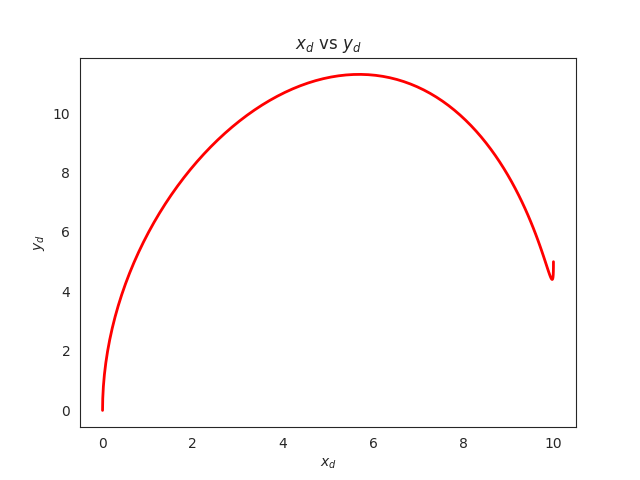
\includegraphics[scale=0.5]{plot.png}
  \caption{Optimized trajectory.\label{fig:plot}}
\end{figure}

\end{document}

